\chapter{Исследовательская часть}

\section{Технические характеристики}

Технические характеристики устройства, на котором выполнялись замеры по времени, представлены далее.

\begin{itemize}
	\item Процессор: Intel(R) Core(TM) i7-1165G7 CPU 2.80 ГГц.
	\item Оперативная память: 15 ГБайт.
	\item Операционная система: Ubuntu 64-разрядная система версии 22.04.3.
\end{itemize}

При замерах времени ноутбук был включен в сеть электропитания и был нагружен только системными приложениями.

\clearpage

\section{Демонстрация работы программы}

На рисунке \ref{img:demonstration} представлена демонстрация работы разработанного приложения для алгоритмов сортировок, у которого имеется консольное меню для выбора запуска одного или всех алгоритмов или процесс замера по времени работы алгоритмов.

\begin{figure}[h]
	\centering
	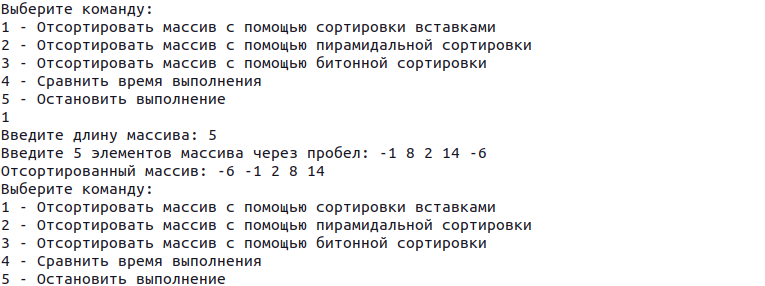
\includegraphics[height=0.35\textheight]{img/example.png}
	\caption{Демонстрация работы программы}
	\label{img:demonstration}
\end{figure}

\section{Временные характеристики}

Результаты эксперимента замеров по времени приведены в таблицах \ref{tbl:time_sort} -- \ref{tbl:time_rsort}.

В таблице \ref{tbl:time_sort} приведены результаты замеров по времени лучшего случая для сортировки вставками и пирамидальной сортировки, то есть при входном массиве отсортированном по возрастанию.
Чтобы сравнить с ними битонную сортировку, использовались только массивы с длиной, равной степенью двойки.

\begin{table}[H]
	\small
	\begin{center}
		\begin{threeparttable}
		\caption{Замеры по времени лучшего случая для сортировок, размер которых от 32 до 1024.}
		\label{tbl:time_sort}
		\begin{tabular}{|r|r|r|r|}
			\hline
			& \multicolumn{3}{c|}{\bfseries Время, мс} \\ \cline{2-4}
			\bfseries Количество элементов & \bfseries Вставками & \bfseries Пирамидальной & \bfseries Битонный
			\csvreader{csv/best.csv}{}
			{\\\hline \csvcoli & \csvcolii & \csvcoliii & \csvcoliv} \\
			\hline
		\end{tabular}
		\end{threeparttable}
	\end{center}
\end{table}

% TODO: посмотреть в справочнике лучший и худший случай для битонной сортировки
По таблице \ref{tbl:time_sort} был построен рисунок \ref{plt:sort_1}, где можно сравнить в лучшем случае сортировки вставками, пирамидальную и битонную.
Исходя из этих данных можно понять, что лучшего всего в этом случае работает пирамидальная сортировка.
При этом разница во времени между пирамидальной сортировкой и сортировкой вставками значительна --- в 1000-3000 раза, а хуже всего работает битонная сортировка --- в 1000-2500 раз медленнее, чем сортировка вставками.

\begin{figure}[H]
	\centering
	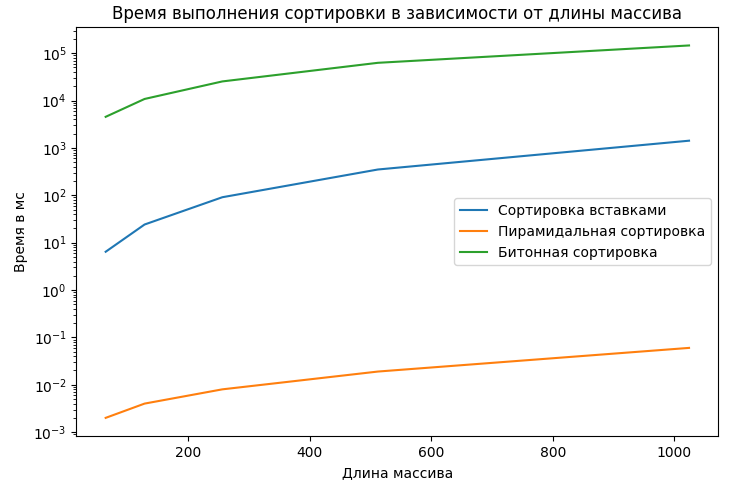
\includegraphics[height=0.28\textheight]{img/best1.png}
	\caption{Сравнение по времени сортировок вставками, пирамидальной и битонной с входным отсортированным по возрастанию массивом}
	\label{plt:sort_1}
\end{figure}

\clearpage

В таблице \ref{tbl:time_random} приведены результаты замеров по времени для сортировки вставками, пирамидальной сортировки и битонной сортировки, где на вход поступает отсортированный по возрастанию массив данных размером, равным степеням двойки от 32 до 1024.

\begin{table}[ht]
	\small
	\begin{center}
		\begin{threeparttable}
		\caption{Замеры по времени, размер которых от 32 до 1024, с входным случайным массивом}
		\label{tbl:time_random}
		\begin{tabular}{|r|r|r|r|}
			\hline
			& \multicolumn{3}{c|}{\bfseries Время, мс} \\ \cline{2-4}
			\bfseries Количество элементов & \bfseries Вставками & \bfseries Пирамидальной & \bfseries Битонной
			\csvreader{csv/random.csv}{}
			{\\\hline \csvcoli & \csvcolii & \csvcoliii & \csvcoliv} \\
			\hline
		\end{tabular}
		\end{threeparttable}
	\end{center}
\end{table}

По таблице \ref{tbl:time_random} были построен рисунук \ref{plt:random1}.
Исходя из этих данных можно понять, что лучшего всего в этом случае работает пирамидальная сортировка.
При этом разница во времени между пирамидальной сортировкой и сортировкой вставками значительна --- в 1000-3000 раза, а хуже всего работает битонная сортировка --- в 1000-2500 раз медленнее, чем сортировка вставками.

\begin{figure}[H]
	\centering
	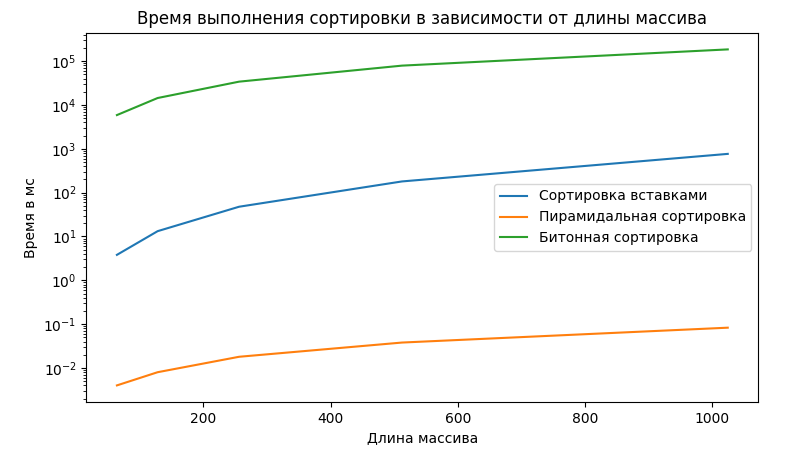
\includegraphics[height=0.28\textheight]{img/random1.png}
	\caption{Сравнение по времени сортировок вставками, пирамидальной и битонной с входным случайным массивом}
	\label{plt:random1}
\end{figure}

\clearpage

В таблице \ref{tbl:time_rsort} приведены результаты замеров худшего случая по времени для сортировки вставками, пирамидальной сортировки и битонной сортировки, то есть для сортировок вставками и пирамидальной это случаи, когда массив отсортирован по убыванию (в обратном порядке сортировки).
При замерах по времени поступал массив размером, равным степеням двойки от 32 до 1024.

\begin{table}[ht]
	\small
	\begin{center}
		\begin{threeparttable}
		\caption{Замеры по времени, размер которых от 32 до 1024, с входным отсортированным массивом по убыванию}
		\label{tbl:time_rsort}
		\begin{tabular}{|r|r|r|r|}
			\hline
			& \multicolumn{3}{c|}{\bfseries Время, мс} \\ \cline{2-4}
			\bfseries Количество элементов & \bfseries Вставками & \bfseries Пирамидальный & \bfseries Битонный
			\csvreader{csv/worst.csv}{}
			{\\\hline \csvcoli & \csvcolii & \csvcoliii & \csvcoliv} \\
			\hline
		\end{tabular}
		\end{threeparttable}
	\end{center}
\end{table}

По таблице \ref{tbl:time_random} были построен рисунок \ref{plt:rsort_1}, в которых сравниваются в худшем случае сортировка вставками и пирамидальная сортировка.
Исходя из этих данных можно понять, что лучшего всего в этом случае работает пирамидальная сортировка.
При этом разница во времени между пирамидальной сортировкой и сортировкой вставками значительна --- в 1000-3000 раза, а хуже всего работает битонная сортировка --- в 1000-2500 раз медленнее, чем сортировка вставками.

\begin{figure}[H]
	\centering
	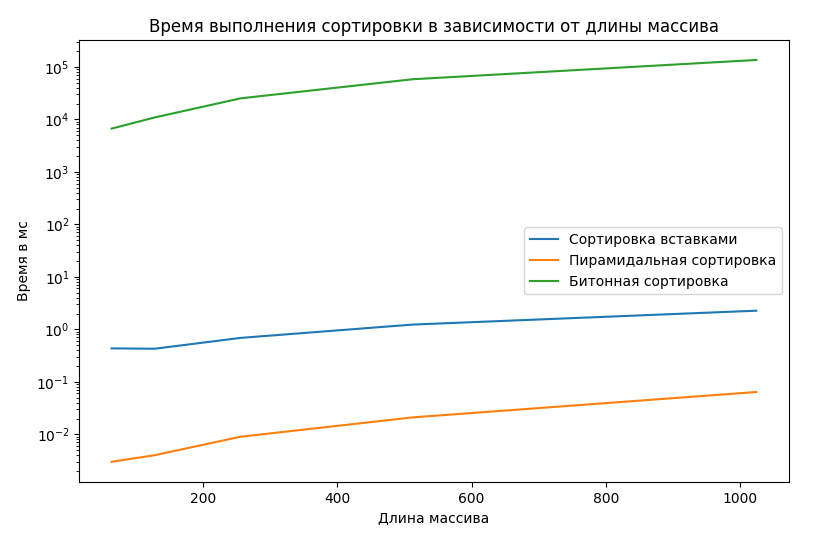
\includegraphics[height=0.28\textheight]{img/worst1.png}
	\caption{Сравнение по времени сортировок вставками, пирамидальной и битонной с входным отсортированным массивом по убыванию}
	\label{plt:rsort_1}
\end{figure}

\clearpage

\section{Вывод}
В данном разделе было произведено сравнение количества затраченного времени вышеизложенных алгоритмов.
Наименее затратным по времени оказалась пирамидальная сортировка для отсортированного массива по возрастанию и пирамидальная сортировка для отсортированного массива по убыванию, а худшей сортировкой оказалась битонная сортировка.

Приведенные временные характеристики показывают, что лучшей сортировкой при работе с массивом является пирамидальная сортировка.
Битонная сортировка же показала худшие результаты по сравнению с сортировкой вставками и пирамидальной, требуя 1000-3000 больше времени в зависимости от входных данных.
